\chapter{Implementation using FEniCS and Firedrake}

In this appendix, the main tools needed for implementing PFEM  in \fenics and \firedrake libraries are illustrated. It is assumed to a recent version of \fenics and \firedrake is available, either through local installation (Anaconda or installation from source for \fenics and virtual Python environment for \firedrake) or through Docker containers. Additional information concerning the installation can be found at \url{https://fenicsproject.org/download/} for \fenics and \url{https://www.firedrakeproject.org/download.html} for \firedrake. \\

This tutorial is by no means a complete introductory tutorial. It is intended to provide the general commands needed for the implementation of PFEM and to highlight similarities and differences between \fenics and \firedrake. For readers interested in a comprehensive documentation, the \fenics developers have written a book to explain the functioning of the library \cite{logg2012}, whereas the \firedrake developers employ illustrative tutorials\footnote{\url{https://www.firedrakeproject.org/documentation.html}}. \\

In this appendix, boxes colored in red are used for \textcolor{red}{\fenics}, cyan for \textcolor{cyan}{\firedrake}, gray for identical commands in both libraries and green for implementations based on \textsc{Scipy}. The \fenics or \firedrake library is assumed to be loaded through the star import:	
\begin{verbatim}
from fenics import *
\end{verbatim}
or
\begin{verbatim}
from firedrake import *
\end{verbatim}
Furthermore, the \textsc{Numpy} library and some method of the \textsc{Scipy} sparse library  are needed\footnote{\url{https://www.scipy.org/}}:
\begin{Verbatim}
import numpy as np
from scipy.sparse import csr_matrix
from scipy.sparse import lil_matrix
from scipy.sparse import vstack, hstack, block_diag
from scipy.sparse.linalg import eigs
\end{Verbatim}
As an illustration we consider the discretization of the Mindlin plate using the CGDG elements  \eqref{eq:CGDG}. We first illustrate how to compute the mass and interconnection matrices. Then, the construction of the boundary control matrix is explained by retrieving a \textsc{Scipy} sparse matrix from the matrix computed by \fenics or \firedrake.

\subsection*{Creation of a mixed function space}
For the discretization of pHs one has to use a mixed function space, i.e. a collection of more than one function space. Consider the creation of the Mindlin plate CGDG elements \eqref{eq:CGDG} on a unit square simplicial mesh with 40 elements per side.
\begin{tcolorbox}[title = Mixed function space in  \fenics, coltitle=black, breakable, size=fbox, boxrule=1pt, pad at break*=1mm, colframe=red, enlarge top by=0.25em, enlarge bottom by=0.5em]
\begin{Verbatim}[tabsize=4]
n_el  = 40
mesh  = UnitSquareMesh(n_el, n_el)
P_w   = FiniteElement('CG', triangle, 1)   	# vertical velocity
P_th  = VectorElement('CG', triangle, 1)   	# angular velocity
P_kap = VectorElement('DG', triangle, 0, dim=3)	# bending momenta			
P_gam = VectorElement('DG', triangle, 0)	# shear stress 
elem  = MixedElement([P_w, P_th, P_kap, P_gam])
V     = FunctionSpace(mesh, elem)
\end{Verbatim}
\end{tcolorbox}
\begin{tcolorbox}[title = Mixed function space in  \firedrake, coltitle=black, breakable, size=fbox, boxrule=1pt, pad at break*=1mm, colframe=cyan, enlarge top by=0.25em, enlarge bottom by=0.5em]
\begin{Verbatim}[tabsize=4]
n_el  = 40
mesh  = UnitSquareMesh(n_el, n_el)
V_w   = FunctionSpace(mesh, "CG", 1)
V_th  = VectorFunctionSpace(mesh, "CG", 1)
V_kap = VectorFunctionSpace(mesh, "DG", 0, dim=3)
V_gam = VectorFunctionSpace(mesh, "DG", 0)
V     = MixedFunctionSpace([V_w, V_th, V_kap, V_gam])
\end{Verbatim}
\end{tcolorbox}
The space $\verb|V_kap|$ has dimension 3 since it corresponds to variable $\bm{E}_\kappa \in \bbR^{2\times 2}_{\text{sym}} \cong  \bbR^3$, ($\cong$ stands for isomorphic).

\subsection*{Definition of variational forms}
The precedent commands create a mixed function space that can be used to construct variational forms trough the Unified Form Language\footnote{\url{https://readthedocs.org/projects/fenics-ufl/downloads/pdf/latest/}} \cite{alnaes2014} (UFL). UFL is a core component of \fenics and has been adopted in \firedrake as well. It is an expressive domain-specific language for abstractly representing (finite element) variational formulations of differential equations. In particular, this language defines a syntax for the integration of variational forms over various domains. \\

Given the previously defined mixed function space, consider the definition of the mass and interconnection variational forms (the implementation is the same in both libraries since UFL is a common component).
 
\begin{tcolorbox}[title = Definition of the variational forms (\fenics \& \firedrake), coltitle=white, breakable, size=fbox, boxrule=1pt, pad at break*=1mm, enlarge top by=0.25em, enlarge bottom by=0.5em]
\begin{Verbatim}[tabsize=4]
# Physical parameters 
E   = 1e12
nu  = 0.3	
rho = 2600
h   = 0.1
k   = 5/6	
G   = E / 2 / (1 + nu)
F   = G * h * k

# Definition of the bending curvature operator
def bending_curv(mom):
	kappa = 12. / (E * h ** 3) * ((1+nu)*mom - nu * Identity(2) * tr(mom))
	return kappa
	
# Test variables
v = TestFunction(V)
v_w, v_th, v_kap, v_gam = split(v)	

# Co-energy variables
e = TrialFunction(V)
e_w, e_th, e_kap, e_gam = split(e)

# Convert the R^3 vector to a symmetric tensor
v_kap = as_tensor([[v_kap[0], v_kap[1]],
				   [v_kap[1], v_kap[2]]])
e_kap = as_tensor([[e_kap[0], e_kap[1]],
				   [e_kap[1], e_kap[2]]])
			
# Energy variables   
a_w   = rho * h * e_w
a_th  = (rho * h ** 3) / 12. * e_th
a_kap = bending_curv(e_kap)
a_gam = 1. / F * e_gam

# Mass bilinear form 
m_form = v_w * a_w * dx + dot(v_th, a_th) * dx + \
		 inner(v_kap, a_kap) * dx + dot(v_gam, a_gam) * dx 

# Interconnection bilinear form
j_form = dot(v_gam, grad(e_w)) * dx - dot(grad(v_w), e_gam) * dx + \
		 inner(v_kap, sym(grad(e_th))) * dx - \
		 inner(sym(grad(v_th)), e_kap) * dx + \
		 dot(v_th, e_gam) * dx - dot(v_gam, e_th) * dx
\end{Verbatim}
\end{tcolorbox}
This sample code highlights the strength of the UFL library. The expressive implementation is really close to the abstract mathematical formulation.

\subsection*{Matrices assemble}
Once the forms have been declared, it is possible to actually construct the associated matrices. Consider the case of a clamped (i.e. Dirichlet) boundary condition. For the CGDG elements a clamped condition corresponds to essential boundary conditions. These are defined in the same way in \fenics and \firedrake
\begin{tcolorbox}[title = Dirichlet boundary conditions (\fenics \& \firedrake), coltitle=white, breakable, size=fbox, boxrule=1pt, pad at break*=1mm, enlarge top by=0.25em, enlarge bottom by=0.5em]
\begin{Verbatim}[tabsize=4]
bcs = []
bcs.append(DirichletBC(V.sub(0), Constant(0.0), "on_boundary"))
bcs.append(DirichletBC(V.sub(1), Constant((0.0, 0.0)), "on_boundary"))
\end{Verbatim}
\end{tcolorbox}
The subspaces \verb|V.sub(0)|, \verb|V.sub(1)| correspond to spaces \verb|V_w|, \verb|V_th| associated to the vertical velocity and the angular velocity, respectively. The boundary conditions can now be incorporated in the matrices. The final assemble of the matrices is achieved in \fenics by the following code snippet.
\begin{tcolorbox}[title = Matrices assemble in  \fenics, coltitle=black, breakable, size=fbox, boxrule=1pt, pad at break*=1mm, colframe=red, enlarge top by=0.25em, enlarge bottom by=0.5em]
\begin{Verbatim}[tabsize=4]
J, M = PETScMatrix(), PETScMatrix()
dummy = v_w * dx
assemble_system(j_form, dummy, bcs, A_tensor=J)
assemble_system(m_form, dummy, bcs, A_tensor=M)
\end{Verbatim}
\end{tcolorbox}
Matrices are first defined as {\sc{PETSc}}\footnote{\url{https://www.mcs.anl.gov/petsc/}} matrices and forms are assembled into it. The boundary conditions have been applied to the stiffness matrix using \verb|assemble_system| so as to preserve symmetry (a dummy right-hand side vector have been introduced to call this function). The same matrices are constructed in \firedrake by the following code
\begin{tcolorbox}[title = Matrices assemble in  \firedrake, coltitle=black, breakable, size=fbox, boxrule=1pt, pad at break*=1mm, colframe=cyan, enlarge top by=0.25em, enlarge bottom by=0.5em]
\begin{Verbatim}[tabsize=4]
J_ass = assemble(j_form, bcs=bcs, mat_type='aij')
M_ass = assemble(m_form, bcs=bcs, mat_type='aij')
J = J_ass.M.handle
M = M_ass.M.handle
\end{Verbatim}
\end{tcolorbox}
The option \verb|mat_type| specifies the desired format for the matrix representation. To get a final {\sc{PETSc}} matrix, the AIJ format is used. The method \verb|M.handle| provide as outputs {\sc{PETSc}} matrices that can be manipulated by the \verb|pesct4py| library\footnote{\url{https://www.mcs.anl.gov/petsc/petsc4py-current/docs/apiref/index.html}}. \\

For what concerns the ordering of the degrees of freedom, \firedrake just piles up the degrees of freedom of each subspace. The final matrices have the same structure as in \eqref{eq:pHfindim_Min_grad}. For \fenics the default option is a not-natural ordering to cluster the non-zero entries closer to the diagonal. A natural ordering can be set by changing the \verb|reorder_dofs_serial| parameter\footnote{\url{https://fenicsproject.discourse.group/t/ordering-of-mixed-elements/946}}.

\subsection*{Eigenvalues computation with SLEPc}
A simple test to assess the validity of the finite element discretization consists in computing the eigenvalues of the matrices, to assess the absence of spurious modes. The {\sc{SLEPc}} library is used to this end \footnote{\url{https://slepc.upv.es/documentation/slepc.pdf}} \cite{hernandez2005slepc}. Since we are interested in the lowest eigenvalues, a shift-and-invert method is used. It is known that for this problem the first normalized eigenfrequencies
\[
\widehat{\omega}_i = \omega_i \; (2(1+\nu)\rho/E)^{1/2}
\]
are close to 1 \cite{dawe1980rayleigh}. Hence, a good choice for the spectral shift is $\sigma = (2(1+\nu)\rho/E)^{-1/2}$.  The following code compute the eigenvalues.
\begin{tcolorbox}[title = Eigenvalues computation in  \fenics, coltitle=black, breakable, size=fbox, boxrule=1pt, pad at break*=1mm, colframe=red, enlarge top by=0.25em, enlarge bottom by=0.5em]
\begin{Verbatim}[tabsize=4]
solver = SLEPcEigenSolver(J, M)
solver.parameters["solver"] = "krylov-schur"
# Set the problem type: the J matrix is not hermitian nor positive.
solver.parameters["problem_type"] = "pos_gen_non_hermitian"
# We look for eigenvalues on the imaginary axis.
solver.parameters["spectrum"] = "target imaginary"
solver.parameters["spectral_transform"] = "shift-and-invert"
solver.parameters["spectral_shift"] = 1/((2*(1+nu)*rho)/E)**0.5
solver.solve(40)
n_conv = solver.get_number_converged()

omega_tilde = []
for i in range(n_conv):
	lam_r, lam_i, psi_r, psi_i = solver.get_eigenpair(i)
	
	# Discard the zero eigenvalues due to the bcs.
	if lam_i > 1e-5:
		omega_tilde.append(lam_i *((2 * (1 + nu) * rho) / E) ** 0.5)
\end{Verbatim}
\end{tcolorbox}
 For \firedrake the equivalent code snippet is the following.
\begin{tcolorbox}[title = Eigenvalues computation in  \firedrake, coltitle=black, breakable, size=fbox, boxrule=1pt, pad at break*=1mm, colframe=cyan, enlarge top by=0.25em, enlarge bottom by=0.5em]
\begin{Verbatim}[tabsize=4]
# Check for SLEPc
from firedrake.petsc import PETSc
try:
	from slepc4py import SLEPc
except ImportError:
	import sys
	warning("Unable to import SLEPc (try firedrake-update --slepc)")
	sys.exit(0)
	
# Options for the solver.
opts = PETSc.Options()
opts.setValue("pos_gen_non_hermitian", None)
opts.setValue("st_pc_factor_shift_type", "NONZERO")
opts.setValue("eps_type", "krylovschur")
opts.setValue("st_type", "sinvert")
opts.setValue("st_shift", 1/(((2*(1+nu)*rho)/E)**0.5))
opts.setValue("eps_target", 1/(((2*(1+nu)*rho)/E)**0.5))

# Construction of the eigensolver.
es = SLEPc.EPS().create(comm=COMM_WORLD)
es.setDimensions(40)
es.setOperators(J, M)
es.setFromOptions()
es.solve()

n_conv = es.getConverged()
psi_r, psi_i = J.getVecs()
omega_tilde = []
for i in range(n_conv):
	lam = es.getEigenpair(i, psi_r, psi_i)
	lam_i = np.imag(lam)
	
	if lam_i > 1e-5:
		omega_tilde.append(lam_i*((2*(1+nu)*rho)/E)**0.5)
\end{Verbatim}
\end{tcolorbox}

In Fig. \ref{fig:EigMin} the 6 first eigenvectors are plotted. The associated eigenvalues are consistent with the results reported in \cite{dawe1980rayleigh}. 

\begin{figure*}[hp]
	\centering
	\subfloat[$\widehat{\omega}_1 = 1.60$]{\includegraphics[width=0.5\linewidth]{appendix/Eig1.eps}%
		\label{fig:Eig1}}
	\hfil
	\subfloat[$\widehat{\omega}_2 = 3.06$]{\includegraphics[width=0.5\linewidth]{appendix/Eig2.eps}%
		\label{fig:Eig2}} \\
	\subfloat[$\widehat{\omega}_3 = 3.07$]{\includegraphics[width=0.5\linewidth]{appendix/Eig3.eps}%
		\label{fig:Eig3}}
	\hfil
	\subfloat[$\widehat{\omega}_4 = 4.31$]{\includegraphics[width=0.5\linewidth]{appendix/Eig4.eps}%
		\label{fig:Eig4}} \\
	\subfloat[$\widehat{\omega}_3 = 5.08$]{\includegraphics[width=0.5\linewidth]{appendix/Eig5.eps}%
		\label{fig:Eig5}}
	\hfil
	\subfloat[$\widehat{\omega}_4 = 5.13$]{\includegraphics[width=0.5\linewidth]{appendix/Eig6.eps}%
		\label{fig:Eig6}}
	\caption{Eigenvectors for the clamped Mindlin plate computed with \firedrake. The eigenfrequencies are normalized $\widetilde{\omega} = \omega((2(1+\nu)\rho/E)^{1/2}$.}
	\label{fig:EigMin}
\end{figure*}



\subsection*{Conversion to \textsc{Scipy} for direct manipulation of the boundary matrices}
If boundary control has to be taken into account, it is preferable to move to \textsc{Scipy} for manipulating and constructing the final matrices. Consider now the case of a Mindlin plate with Neumann boundary control. The construction of the mass and interconnection matrices is the same, without imposing any boundary conditions. For the boundary variables we choose Lagrange polynomials of order~1. 

\begin{remark}[Construction of the $\mathbf{B}$ matrix]\label{rmk:Bmatrix}
Notice that \fenics and \firedrake do not support Function spaces defined on the boundary. It is therefore necessary to construct the $\mathbf{B}$ matrix using function defined on the domain and then eliminate the useless columns. First, we show how to construct the $\mathbf{B}$ matrix cointaing all degrees of freedom. Later on, the extraction of the boundary degrees of freedom is illustrated using \textsc{Scipy}. 
\end{remark}

\begin{tcolorbox}[title = Control matrix construction in  \fenics, coltitle=black, breakable, size=fbox, boxrule=1pt, pad at break*=1mm, colframe=red, enlarge top by=0.25em, enlarge bottom by=0.5em]
\begin{Verbatim}[tabsize=4]
P_qn  = FiniteElement('CG', triangle, 1)   # shear force
P_Mnn = FiniteElement('CG', triangle, 1)   # flexural momentum
P_Mns = FiniteElement('CG', triangle, 1)   # torsional momentum
elem  = MixedElement([P_qn, P_Mnn, P_Mns])
 
V_u   = FunctionSpace(mesh, elem)
q_n, M_nn, M_ns = TrialFunction(V_u)

n_ver = FacetNormal(mesh)  
s_ver = as_vector([-n_ver[1], n_ver[0]])

b_form = v_w * q_n * ds + dot(v_th, n_ver) * M_nn * ds + \
		 dot(v_th, s_ver) * M_ns * ds	 
B_petsc = PETScMatrix()
assemble(b_form, B_petsc)
B = B_petsc.mat()
\end{Verbatim}
\end{tcolorbox}	
The method \verb|mat()| in \fenics provides a PETCs matrix manageable by \verb|petsc4py|, similarly to the method \verb|M.handle| in \firedrake.

\begin{tcolorbox}[title = Control matrix construction in  \firedrake, coltitle=black, breakable, size=fbox, boxrule=1pt, pad at break*=1mm, colframe=cyan, enlarge top by=0.25em, enlarge bottom by=0.5em]
\begin{Verbatim}[tabsize=4]
V_qn  = FunctionSpace(mesh, 'CG', 1)
V_Mnn = FunctionSpace(mesh, 'CG', 1)
V_Mns = FunctionSpace(mesh, 'CG', 1)

V_u = V_qn * V_Mnn * V_Mns
q_n, M_nn, M_ns = TrialFunction(V_u)

n_ver = FacetNormal(mesh)  # outward normal to the boundary
s_ver = as_vector([-n_ver[1], n_ver[0]])  # tangent versor to the boundary

b_form = v_w * q_n * ds + dot(v_th, n_ver) * M_nn * ds + \
		 dot(v_th, s_ver) * M_ns * ds
B_ass = assemble(b_form, mat_type='aij')
B = B_ass.M.handle
\end{Verbatim}
\end{tcolorbox}

The matrix \verb|B| computed with \fenics and \firedrake has now the type \verb|petsc4py.PETSc.Mat| and can be converted to a \textsc{Scipy} sparse CSR matrix (compressed sparse row format). As anticipated in Remark \ref{rmk:Bmatrix}, the zero columns associated with interior degrees of freedom have to be removed from the matrix.
\begin{tcolorbox}[title = Construction of the final $\mathbf{B}$ matrix (\textsc{Scipy}), coltitle=black, breakable, size=fbox, boxrule=1pt, pad at break*=1mm, colframe=green, enlarge top by=0.25em, enlarge bottom by=0.5em]
\begin{Verbatim}[tabsize=4]
# Conversion to CSR scipy format
B_scipy_cols = csr_matrix(B.getValuesCSR()[::-1])

# Non zero rows and columns
rows, cols = csr_matrix.nonzero(B_scipy_cols)

# Indexes of non zero columns
set_cols = np.array(list(set(cols)))

# Number of non zero columns (i.e. number of inputs)
n_u = len(set(cols))

# Initialization of the final matrix in lil folmat
# for efficient incremental construction.
B_scipy = lil_matrix((V.dim(), n_u))

for r, c in zip(rows, cols):
	# Column index in the final matrix
	ind_col = np.where(set_cols == c)[0]
	
	# Fill the matrix with the values
	B_scipy[r, ind_col] = B_scipy_cols[r, c]
	
# Convert to csr format
B_scipy.tocsr()	
\end{Verbatim}
\end{tcolorbox}
Similarly \textsc{Scipy} matrices in CSR format can be obtained for the mass $\mathbf{M}$ and interconnection $\mathbf{J}$ matrix, thus obtaining the final boundary controlled system
\begin{equation*}
\mathbf{M} \dot{\mathbf{e}} = \mathbf{J} \mathbf{e} + \mathbf{B} \mathbf{u}.
\end{equation*}
This system can then be simulated using time integrator libraries available in \textsc{Scipy}\footnote{\url{https://docs.scipy.org/doc/scipy/reference/integrate.html}}.

\subsection*{Stability check of the boundary subspace}
To check if the discretization of the boundary variable is appropriate, one can solve the eigenvalues problem
\begin{equation*}
	\begin{bmatrix}
	\mathbf{M} & \mathbf{0} \\
	\mathbf{0} & \mathbf{0}
	\end{bmatrix}
	\begin{pmatrix}
	\bm{\psi}_e^i \\
	\bm{\psi}_\lambda^i
	\end{pmatrix} j \omega_i  = 
	\begin{bmatrix}
	\mathbf{J} & \mathbf{B} \\
	-\mathbf{B}^\top & \mathbf{0}
	\end{bmatrix}
	\begin{pmatrix}
	\bm{\psi}_e^i \\
	\bm{\psi}_\lambda^i
	\end{pmatrix},
\end{equation*}
and check the consistency of the eigenvalues, i.e. no spurious modes appear.
\begin{tcolorbox}[title = Eigenvalues computation using Lagrange multipliers (\textsc{Scipy}), coltitle=black, breakable, size=fbox, boxrule=1pt, pad at break*=1mm, colframe=green, enlarge top by=0.25em, enlarge bottom by=0.5em]
\begin{Verbatim}[tabsize=4]
# Conversion to scipy CSR matrices 
# Important: no boundary conditions imposed
J_scipy = csr_matrix(J.getValuesCSR()[::-1])  # for fenics J.mat() 
M_scipy = csr_matrix(M.getValuesCSR()[::-1])  # for fenics M.mat() 

Z_mat = csr_matrix((n_u, n_u))
J_aug = vstack((hstack((J_scipy, B_scipy)), hstack((-B_scipy.T, Z_mat))))
M_aug = block_diag((M_scipy, Z_mat))

# Shift value
shift = 1/(((2*(1+nu)*rho)/E)**0.5)
# Resolution of the eigenproblem
eigenvalues, eigvectors = eigs(J_aug, k=40, M=M_aug,\
	 					  sigma=shift, which='LM', tol=1e-6)

omega_all = np.imag(eigenvalues)
index = omega_all >= 1e-5
omega = omega_all[index]
omega.sort()

omega_tilde = omega*((2*(1+nu)*rho)/E)**0.5
\end{Verbatim}
\end{tcolorbox}

The following values are obtained 
\begin{align*}
\widehat{\omega}_1 = 1.59, \qquad\qquad \widehat{\omega}_2 = 3.04, \qquad\qquad \widehat{\omega}_3 = 3.06, \\
\widehat{\omega}_4 = 4.29, \qquad\qquad \widehat{\omega}_5 = 5.05, \qquad\qquad \widehat{\omega}_6 = 5.10. \\
\end{align*}
Since no spurious eigenvalues occur, it is legit to assume that the Lagrange multiplier subspace is a stable one (among others). This is just an heuristic reasoning, since the rigorous mathematical justification of the boundary subspace stability comes from the fulfillment of the \textit{inf-sup} condition.

\subsection*{Concluding remarks}
This appendix provides all the tools needed for constructing of the matrices and for handling a uniform boundary conditions. If one has to consider mixed boundary conditions, the boundary forms and Dirichlet conditions have to be defined on a subset of the boundary (consult \url{https://fenicsproject.org/pub/tutorial/sphinx1/._ftut1005.html} for an explanation in \fenics and \url{https://www.firedrakeproject.org/variational-problems.html} for \firedrake). 